\documentclass[11pt,a4paper]{jsarticle}

\usepackage{amsmath,amssymb}
\usepackage[dvipdfmx]{graphicx}
\usepackage{amsmath}
\usepackage{bm}
\usepackage{multirow}
\usepackage{fancyhdr}
\usepackage{listings}

\setlength{\textheight}{\paperheight}
\setlength{\topmargin}{4.6truemm} % 30mm(=1.0in+4.6mm)
\addtolength{\topmargin}{-\headheight}
\addtolength{\topmargin}{-\headsep}
\addtolength{\textheight}{-60truemm}

\setlength{\textwidth}{\paperwidth}
\setlength{\oddsidemargin}{-0.4truemm} % 25mm(=1.0in-0.4mm)
\setlength{\evensidemargin}{-0.4truemm}
\addtolength{\textwidth}{-50truemm}

\pagestyle{fancy}
\rhead{\thepage}
\lhead{}
\cfoot{}

\renewcommand{\theequation}{\arabic{section}.\arabic{equation}}
\renewcommand{\thefigure}{\thesection.\arabic{figure}}
\renewcommand{\thetable}{\thesection.\arabic{table}}
\renewcommand{\lstlistingname}{ソースコード}
\renewcommand{\headrulewidth}{0mm} % fancy

\lstset{
  basicstyle={\ttfamily \small},
  frame=trBL,
  numbers=left,
  numberstyle={\ttfamily \small},
  breaklines=true,
}


\def\exptname{6\hspace{5mm}レベル系の同定}
\def\exptdate{2016年05月31日}
\def\submission{2016年06月07日\\ \hspace{19mm}2016年06月14日}

\pagestyle{fancy}
\rhead{\thepage}
\lhead{}
\cfoot{}

\renewcommand{\thepage}{再\arabic{page}}
\renewcommand{\headrulewidth}{0mm}

\begin{document}

\begin{titlepage}
  \vspace*{30mm}
  \begin{center}
    {\huge 制御工学実験 I\hspace{-0.1mm}I \\}
    \vspace{5mm}
    {\Huge \exptname \\}
    \vspace{20mm}
    {\Large 実験日:\exptdate \\}
    {\Large 提出日:\submission \\}
  \end{center}
  \vspace{25mm}
  \begin{flushright}
    {\LARGE 九州工業大学 工学部 \\}
    {\LARGE 機械知能工学科 知能制御工学コース \\}
    \vspace{10mm}
    {\Large     報告者:{\large 14104131} \hspace{1mm} 山崎 達也  \\}
    {\Large 共同実験者:{\large 14104014} \hspace{1mm} 岩永 大樹  \\
                        {\large 14104051} \hspace{1mm} 酒井 佑樹  \\
                        {\large 14104086} \hspace{1mm} 徳田 あかり \\}
  \end{flushright}
\end{titlepage}


\section{実験目的}
  \setcounter{equation}{0}
  \setcounter{figure}{0}
  \setcounter{table}{0}

  制御対象は,サーボ系とプロセス系の二種に分類できる.
  ここでは,過渡応答が遅いプロセス系を取り上げ,
  流入量および水位をそれぞれ入力および出力とした制御対象の同定実験を行い,
  プロセス系の理解を深める.\\

\section{原理}
  \setcounter{equation}{0}
  \setcounter{figure}{0}
  \setcounter{table}{0}

  まず,図\ref{fig:model}に本実験で用いるレベル系のモデルを示す.
  ただし,図の記号は
  \begin{description}
    \setlength{\leftskip}{10mm}
    \item [$u$]   \hspace{-5mm} タンク1への流入量
    \item [$q_i$] \hspace{-5mm} タンクiからの流出量($i = 1,2$)
    \item [$h_i$] \hspace{-5mm} タンクiの水位($i = 1,2$)
    \item [$A_i$] \hspace{-5mm} タンクiの断面積($i = 1,2$)
    \item [$R_i$] \hspace{-5mm} 流体抵抗($i = 1,2$)
  \end{description}
  を意味する.
  
  \begin{figure}[b]
    \begin{center}
      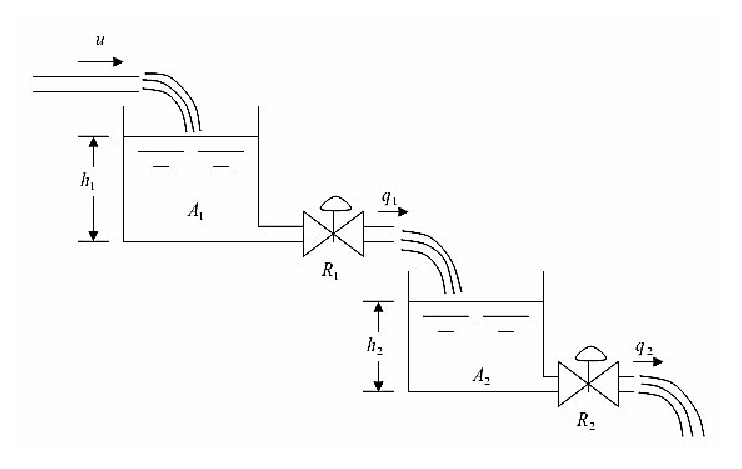
\includegraphics[width=0.8\hsize]{./img/system_model.eps}
    \end{center}
    \caption{レベル系}
    \label{fig:model}
  \end{figure}
  
  本実験では,タンク1への流入量$u$を入力とし,
  タンク2の水位$h_2$を出力とする制御対象の同定を行う.
  制御対象への伝達関数は
  \begin{equation}
    \frac{H_2(s)}{U(s)} = \frac{R_2}{(1 + A_1 R_1 s)(1 + A_2 R_2 s)}
  \end{equation}
  となる.
  したがって,対象とする系は二次遅れ系である.
  ただし,式(2.1)の$U(s)$及び$H_2(2)$は,
  それぞれ$u$及び$h_2$に対応するラプラス変換後の変数である.
  
  次に,二次遅れ系のゲイン及び二つの時定数の決定法を述べる.
  まず,ゲイン$K$,二つの時定数$T_1$,$T_2$の二次遅れ系
  \begin{equation}
    G(s) = \frac{H(s)}{U(s)} = \frac{K}{(1 + T_1 s)(1 + T_2 s)}
  \end{equation}
  に,大きさ$r$のステップ入力を加えた時の時間応答$h(t)$は\\
  \begin{equation}
    h(t) = r K \biggl( 1 + \frac{T_1}{T_2 - T_1} e^{- \frac{t}{T_1}}
                         - \frac{T_2}{T_2 - T_1} e^{- \frac{t}{T_2}} \biggr)
  \end{equation}
  となり,また応答曲線は図\ref{fig:responce}のようになる.
  ただし,図の点$C = (t_c,h(t_c))$は式(2.3)の変曲点であり,
  点$A = (t_a,h_a)$及び点$B = (t_b,h_b)$はそれぞれ変曲点における接線が
  $h(t) = 0$もしくは$h(\infty)$と交わる点,
  また,$T_A = t_b - t_a$,$T_C = t_b - t_c$である.
  
  \begin{figure}[b]
    \begin{center}
      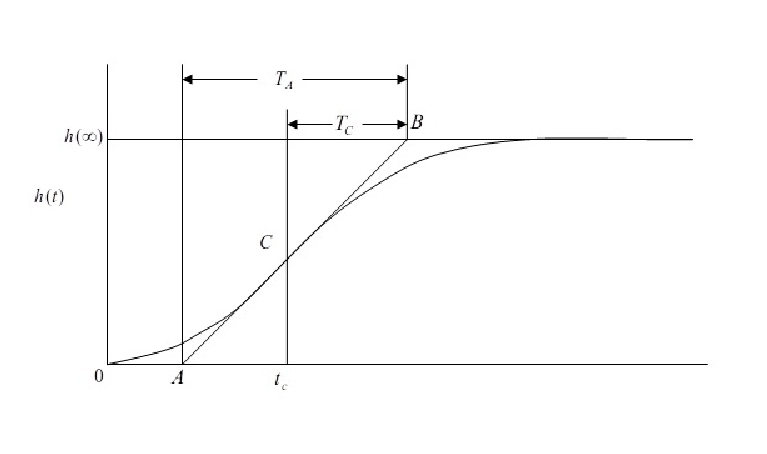
\includegraphics[width=0.9\hsize]{./img/step_responce.eps}
    \end{center}
    \caption{2次遅れ系のステップ応答}
    \label{fig:responce}
  \end{figure}
  
  次に,式(2.3)より次の二式を得る.
  \begin{eqnarray}
    \dot h(t) &=& \frac{r K}{T_2 - T_1} \biggl( - e^{- \frac{t}{T_1}} + e^{- \frac{t}{T_2}} \biggr) \\
    \ddot h(t) &=& \frac{r K}{T_2 - T_1} \biggl( \frac{1}{T_1} e^{- \frac{t}{T_1}} - \frac{1}{T_2} e^{- \frac{t}{T_2}} \biggr)
  \end{eqnarray}
  ここで,$\ddot h(t_c) = 0$より
  \begin{equation}
    T_2 e^{- \frac{t_c}{T_1}} = T_1 e^{- \frac{t_c}{T_2}}
  \end{equation}
  であるので,
  \begin{equation}
    t_c = \ln{\biggl( \frac{T_2}{T_1} \biggr) ^{\frac{T_1 T_2}{T_2 - T_1}}}
  \end{equation}
  を得る.
  
  さらに,接線をAB,CDの二つの直線に分け,
  それぞれの直線の傾きについて考えると,
  式(2.4)と図\ref{fig:responce}より,次の二式を得る.
  \begin{eqnarray}
    \frac{r K}{T_2 - T_1} \biggl( - e^{- \frac{t_c}{T_1}} + e^{- \frac{t_c}{T_2}} \biggr) &=& \frac{r K}{T_A} \\
    \frac{r K - h(t_c)}{T_C} &=& \frac{r K}{T_A}
  \end{eqnarray}
  式(2.6),(2.8)より
  \begin{equation}
    \frac{T_A}{T_1} e^{- \frac{t_c}{T_1}} = 1
  \end{equation}
  となり,式(2.10)に式(2.7)を代入すると次式を得る.
  \begin{equation}
    \frac{T_A}{T_1} \biggl( \frac{T_2}{T_1} \biggr) ^{- \frac{T_2}{T_2 - T_1}} = 1
  \end{equation}
  また,式(2.3),(2.8),(2.9)より,
  \begin{equation}
    T_2 e^{- \frac{t_c}{T_2}} - T_1 e^{- \frac{t_c}{T_1}} = T_C e^{- \frac{t_c}{T_2}} - T_C e^{- \frac{t_c}{T_1}}
  \end{equation}
  となるので,式(2.12)に式(2.6)を代入すると次式を得る.
  \begin{equation}
    T_2 + T_1 = T_C
  \end{equation}
  したがって,式(2.11),(2.13)を用いて,
  $T_A$,$T_C$から$T_1$,$T_2$を求める事が出来る.
  式(2.11),(2.13)より
  \begin{eqnarray}
    \frac{T_A}{T_1} \biggl( \frac{\frac{T_2}{T_A}}{\frac{T_1}{T_A}} \biggr) ^{\frac{\frac{T_2}{T_A}}{\frac{T_2}{T_A} - \frac{T_1}{T_A}}} = 1 \\
    \frac{T_C}{T_A} = \frac{T_1}{T_A} + \frac{T_2}{T_A}
  \end{eqnarray}
  を得るので,
  \begin{equation}
    x \equiv \frac{T_1}{T_A}, \hspace{5mm}
    y \equiv \frac{T_2}{T_A}, \hspace{5mm}
    \alpha \equiv \frac{T_C}{T_A}, \hspace{5mm}
  \end{equation}
  と定義すると,式(2.14),(2.15)は,
  \begin{eqnarray}
    \frac{1}{x} \biggl( \frac{y}{x} \biggr) ^{- \frac{y}{y - x}} = 1 \\
    \alpha = x + y
  \end{eqnarray}
  となる.また,式(2.17)より
  \begin{equation}
    x \log{x} = y \log{y}
  \end{equation}
  を得る.この式(2.19)のデータを表\ref{tab:log}に示す.

  \begin{table}[b] 
  \begin{center}
    \caption{式(2.19)のデータ}
    \begin{tabular}{|c|c|} \hline
      $x$ & $y$   \\ \hline \hline
      0   & 1     \\ \hline
      0.1 & 0.73  \\ \hline
      0.2 & 0.57  \\ \hline
      0.3 & 0.44  \\ \hline
      0.4 & 0.34  \\ \hline
      0.5 & 0.25  \\ \hline
      0.6 & 0.18  \\ \hline
      0.7 & 0.12  \\ \hline
      0.8 & 0.065 \\ \hline
      0.9 & 0.025 \\ \hline
      1   & 0     \\ \hline
    \end{tabular}
    \label{tab:log}
  \end{center}
\end{table}


  式(2.18)の$\alpha$が与えられれば,図\ref{fig:log}に示すように,
  式(2.18)と式(2.19)の交点のx座標$x_1$,$x_2$が得られる.
  したがって,$x_1$,$x_2$を用いることにより,
  式(2.16)より制御対象の二つの時定数$T_1$,$T_2$を求めることが出来る.\\
  
  \begin{figure}[b]
    \begin{center}
      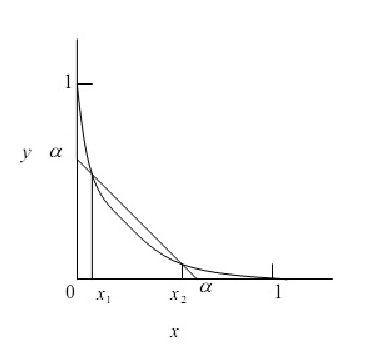
\includegraphics[width=0.5\hsize]{./img/log_relation.eps}
    \end{center}
    \caption{式(2.18)と式(2.19)の関係}
    \label{fig:log}
  \end{figure}

\section{実験装置}
  \setcounter{equation}{0}
  \setcounter{figure}{0}
  \setcounter{table}{0}
  
  まず,図\ref{fig:config}及び表\ref{tab:spec}にレベル実験装置の構成及び仕様を示す.

  \begin{table}[h]
  \begin{center}
    \caption{装置の仕様}
    \begin{tabular}{l|c|p{100mm}} \hline
      装置           & 数 & 仕様 \\ \hline
      タンク1        & 1  & 高さ$1000\,\mathrm{[mm]}$,内径$220\,\mathrm{[mm]}$ \\ \hline
      タンク2        & 1  & 高さ$1500\,\mathrm{[mm]}$,内径$320\,\mathrm{[mm]}$ \\ \hline
      電流比例制御弁 & 3  & 弁開度信号入力:$4〜20\,\mathrm{[mA]}$,全開-全閉時間:$17\,\mathrm{[s]}$以下,\newline 電源:$24\,\mathrm{[VDC]} \pm 10 \%$ \\ \hline
      流量計         & 3  & オープンコレクタ出力,$0.1\,\mathrm{[l/Pulse]}$ \\ \hline
      差圧変換器     & 2  & 容量:$200\,\mathrm{[gf/cm^2]}$ \\ \hline
      A/D変換ボード  & 1  & 入力:8CH,$0〜10\,\mathrm{[V]}$,分解能:$12\,\mathrm{[bit]}$ \\ \hline
      D/A変換ボード  & 1  & 出力:4CH,$4〜20\,\mathrm{[mA]}$,分解能:$12\,\mathrm{[bit]}$,変換速度:$10\,\mathrm{[\mu s/CH]}$ \\ \hline
      パルスカウンタ & 1  & 4CH,$24\,\mathrm{[bit]}$ up/down counter,外部入力:非絶縁TTL入力 \\ \hline
      コンピュータ   & 1  & NEC PC9801RX \\ \hline
    \end{tabular}
    \label{tab:spec}
  \end{center}
\end{table}


  計算機からD/A変換器を介して入力される電流値によって制御バルブMV1の開度が変化し,
  このバルブ開度に対応した流量の水がタンク1に入り
  手動バルブを介してタンク2に流入する.
  また,タンク2から制御バルブMV3を介して水が排出される.
  これら入出流量に依存するタンクの水位は差圧変換器によって計測され,
  D/A変換器を介して計算機に伝送される.\\
  
  \begin{figure}[b]
    \begin{center}
      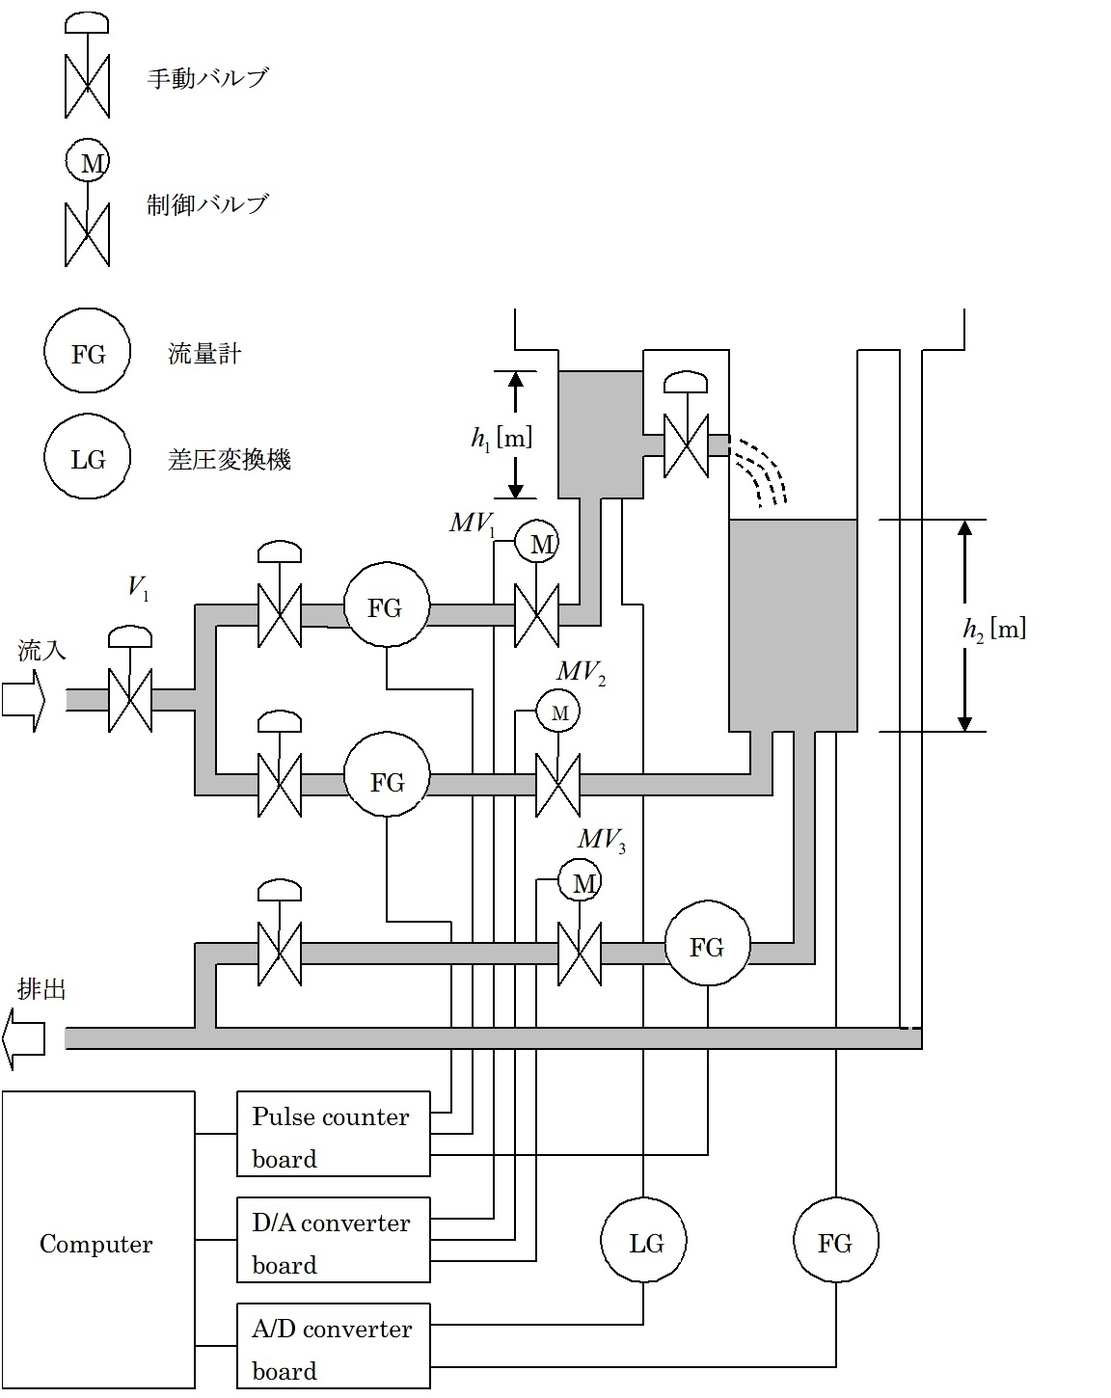
\includegraphics[width=0.7\hsize]{./img/system_config.eps}
    \end{center}
    \caption{実験装置の構成}
    \label{fig:config}
  \end{figure}

\section{実験方法}
  \setcounter{equation}{0}
  \setcounter{figure}{0}
  \setcounter{table}{0}
  
  \subsection{実験準備}
    以下の手順で実験準備を行った.
    ただし,以下の手順1から5は実験指導担当者が行った.
    \begin{enumerate}
      \item 配電盤のレベル系のスイッチを入れる.
      \item コンピュータの電源を入れる.
      \item 実験装置の電源スイッチを入れる.
      \item 給水用バルブ$V_1$を開く.
      \item 実験用プログラムを起動して以下の操作を行う.
            本実験では\texttt{\~{}/exp3}に格納されている下記の2種のプログラムを使用する.
        \begin{enumerate}
          \setlength{\leftskip}{5mm}
          \item \texttt{expapp}:差圧変換器特性の調査実験と流量の調整,タンク2の水抜きを行う.
          \item \texttt{step}:開ループ実験用プログラム.
        \end{enumerate}
      \item プログラム\texttt{expapp}を実行し以下の操作を行う.
            また,操作用コンピュータのディスプレイに表示される図中の記号の意味を
            表\ref{tab:display}に示す.
        \begin{enumerate}
          \setlength{\leftskip}{5mm}
          \item 排水用電磁弁MV3への入力を$20 \, \mathrm{[mA]}$とし全開にする.
          \item 入水用電磁弁MV1への入力を$20 \, \mathrm{[mA]}$とし全開にする.
          \item 流量計の指示値が$30 \, \mathrm{[l/min]}$になるように手動でバルブ$V_1$を調整する.
        \end{enumerate}
    \end{enumerate}
    
    \begin{table}[h]
  \begin{center}
    \caption{\texttt{expapp}における表示の意味}
    \begin{tabular}{c|l|l} \hline
      表記                      & 意味                              & 備考 \\ \hline
      MV1                       & タンク1注水用電磁バルブ指令電流値 & $4 \,\mathrm{[mA]}$から$20 \,\mathrm{[mA]}$ \\ \hline
      MV2                       & タンク2注水用電磁バルブ指令電流値 & $4 \,\mathrm{[mA]}$から$20 \,\mathrm{[mA]}$ \\ \hline
      MV3                       & タンク2排水用電磁バルブ指令電流値 & $4 \,\mathrm{[mA]}$から$20 \,\mathrm{[mA]}$ \\ \hline
      SAMPLING                  & サンプリング時間                  & $1 \,\mathrm{[s]}$から$3 \,\mathrm{[s]}$まで三段階で設定可能 \\ \hline
      APPLY                     & 設定値の変更を適用                & \\ \hline
      SV$\ast \,\mathrm{[mA]}$  & 電磁バルブ指令電流の設定値        & 実験前に表示 \\ \hline
      PV$\ast \,\mathrm{[mA]}$  & 電磁バルブ指令電流の現在地        & 実験中に表示 \\ \hline
      $\ast \,\mathrm{[l/min]}$ & 流量値                            & \\ \hline
      $\ast \,\mathrm{[V]}$     & 差圧変換器出力                    & \\ \hline
      IN                        & 入水経路                          & \\ \hline
      OUT                       & 排水経路                          & \\ \hline
    \end{tabular}
    \label{tab:display}
  \end{center}
\end{table}

  
  \subsection{差圧変換器特性の調査実験}
    以下の手順で差圧変換器特性の調査実験を行った.
    以降,この実験を実験1と呼称する.
    \begin{enumerate}
      \item プログラム\texttt{expapp}を起動する.
      \item タンク2の定常水位が目的の初期水位となるよう入水用制御弁MV2を調整する.
      \item 目的の定常水位におけるタンク2の差圧変換器出力電圧を記録する.
      \item 手順(2)と(3)を水位がおよそ$60 \, \mathrm{[cm]}$となるまで繰り返す.
      \item 差圧変換器の出力電圧と水位の関係のグラフを描く.
    \end{enumerate}
  
  \subsection{ステップ応答実験}
    以下の手順でステップ応答実験を行った.
    以降,この実験を実験2と呼称する.
    \begin{enumerate}
      \item プログラム\texttt{step}を起動する.
      \item プログラムの指示に従い(1)制御弁の初期値,(2)変化量,(3)サンプリング周期を入力する.
      \item \texttt{[APPLY AND START]}をクリックして実験を開始する.
      \item タンク2の水位が定常値に収束した後に\texttt{[Recording Start]}をクリックする.
            10サンプルステップの後に手順(2)で与えた変化量の値だけさらに制御弁が開き,
            タンク2の差圧変換器出力の計測が開始される.
      \item 差圧変換器出力が定常値に収束した後に\texttt{[STOP]}をクリックし,データを保存する.
    \end{enumerate}

\section{実験結果}
  \setcounter{equation}{0}
  \setcounter{figure}{0}
  \setcounter{table}{0}

  実験1,実験2について,それぞれの結果を以下に示す.

  \subsection{実験1:差圧変換器特性}
    タンク2の水位と差圧変換器の出力電圧を$2 \,\mathrm{[cm]}$から
    $57 \,\mathrm{[cm]}$まで$5 \,\mathrm{[cm]}$刻みで計測した.
    得られたデータを表\ref{tab:data1}に示し,またそのデータからプロットした
    差圧変換器出力-タンク水位のグラフを図\ref{fig:data1}に示す.
    
    \begin{table}[b]
  \begin{center}
    \caption{実験1より得られたデータ}
    \begin{tabular}{|c|c|} \hline
タンク水位$\mathrm{[cm]}$ & 差圧変換器出力$\mathrm{[V]}$ \\ \hline \hline
2  & 0.061 \\ \hline
7	 & 0.579 \\ \hline 
12 & 1.170 \\ \hline 
17 & 1.678 \\ \hline 
22 & 2.190 \\ \hline 
27 & 2.708 \\ \hline 
32 & 3.236 \\ \hline 
37 & 3.753 \\ \hline 
42 & 4.295 \\ \hline 
47 & 4.828 \\ \hline 
52 & 5.365 \\ \hline 
57 & 5.907 \\ \hline 
    \end{tabular}
    \label{tab:data1}
  \end{center}
\end{table}

    
    \begin{figure}[b]
      \begin{center}
        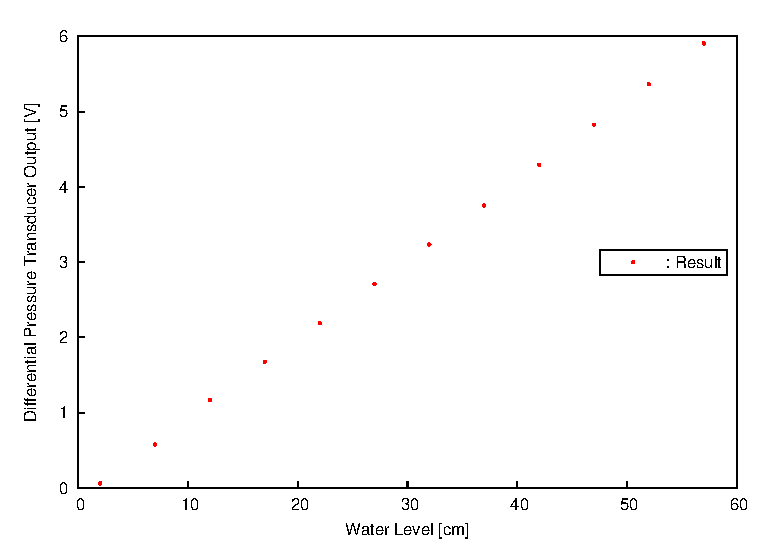
\includegraphics[width=0.9\hsize]{./fig/data1.eps}
      \end{center}
      \caption{実験1:差圧変換器出力-タンク水位のグラフ}
      \label{fig:data1}
    \end{figure}
  
  \subsection{実験2:ステップ応答}
    制御弁の初期値$8 \,\mathrm{[mA]}$,変化量$1 \,\mathrm{[mA]}$,
    サンプリング周期$5 \,\mathrm{[sec]}$として
    タンク2への流入量及び差圧変換器の出力を計測した.
    得られたデータを表\ref{tab:data2}に示し,またそのデータからプロットした
    流入量-時間のグラフを図\ref{fig:data2inflow}に,
    差圧変換器出力-時間のグラフを図\ref{fig:data2dpt}に示す.
    なお,表\ref{tab:data2}に関しては,
    総計測時間が30分を超えデータ量が膨大であったため,
    表では100秒毎のデータに改めている.
    
    \begin{table}[b]
  \begin{center}
    \caption{実験2より得られたデータ}
    \begin{tabular}{|c|c|c|} \hline
      時間$\mathrm{[5sec]}$ & 流入量$\mathrm{[l/min]}$ & 差圧変換器出力$\mathrm{[V]}$ \\ \hline \hline
      0.000   & 16.800   & 1.707 \\ \hline
      20.000  & 24.000   & 1.932 \\ \hline
      40.000  & 24.000   & 2.742 \\ \hline
      60.000  & 24.000   & 3.475 \\ \hline
      80.000  & 24.000   & 3.998 \\ \hline
      100.000	& 24.000   & 4.354 \\ \hline
      120.000	& 24.000   & 4.584 \\ \hline
      140.000	& 24.000   & 4.745 \\ \hline
      160.000	& 24.000   & 4.842 \\ \hline
      180.000	& 24.000   & 4.906 \\ \hline
      200.000	& 22.800   & 4.950 \\ \hline
      220.000	& 22.800   & 4.979 \\ \hline
      240.000	& 22.800   & 5.013 \\ \hline
      260.000	& 24.000   & 5.013 \\ \hline
      280.000	& 22.800   & 5.033 \\ \hline
      300.000	& 22.800   & 5.053 \\ \hline
      320.000	& 24.000   & 5.053 \\ \hline
      340.000	& 24.000   & 5.057 \\ \hline
      360.000	& 22.800   & 5.043 \\ \hline
      380.000	& 24.000   & 5.038 \\ \hline
      400.000	& 24.000   & 5.033 \\ \hline
      420.000	& 22.800   & 5.043 \\ \hline
    \end{tabular}
    \label{tab:data2}
  \end{center}
\end{table}

    
    \begin{figure}[b]
      \begin{center}
        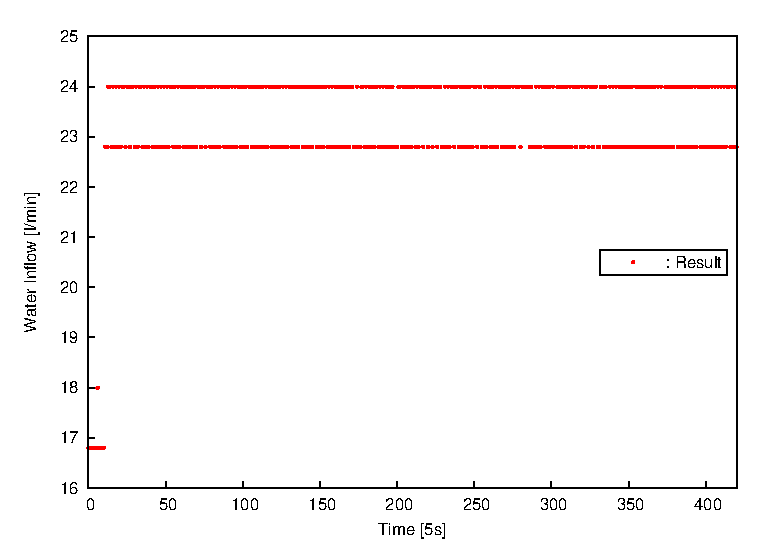
\includegraphics[width=0.9\hsize]{./fig/data2inflow.eps}
      \end{center}
      \caption{実験2:流入量-時間のグラフ}
      \label{fig:data2inflow}
    \end{figure}
    
    \begin{figure}[b]
      \begin{center}
        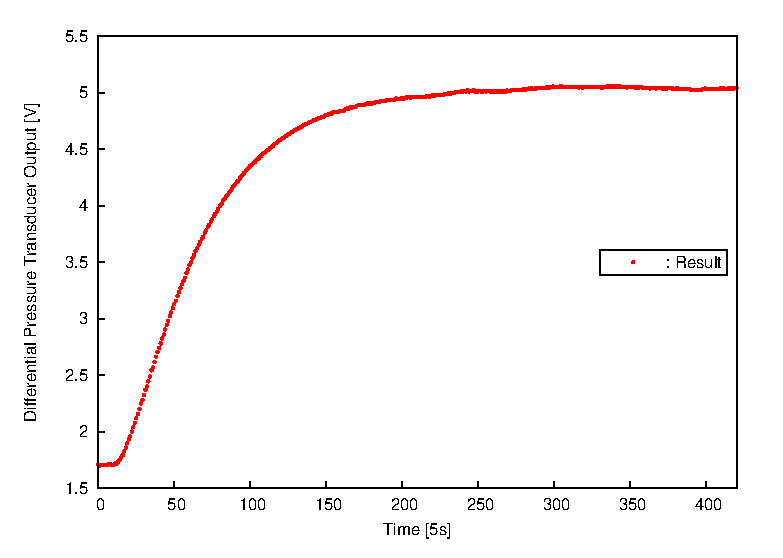
\includegraphics[width=0.9\hsize]{./fig/data2dpt.eps}
      \end{center}
      \caption{実験2:差圧変換器出力-時間のグラフ}
      \label{fig:data2dpt}
    \end{figure}

\section{課題と考察}
  \setcounter{equation}{0}
  \setcounter{figure}{0}
  \setcounter{table}{0}

  \subsection{差圧変換器特性と水位の関係式}
    実験1の結果から,最小二乗法を用いて差圧変換器-水位特性の関係式を求める.
    図\ref{fig:data1}のグラフについて$y = a x + b$とおくと,
    最小二乗法より$a$,$b$はそれぞれ以下のように表せる.
    \begin{eqnarray}
      a &=& \cfrac{n \Sigma x_i y_i - \Sigma x_i \Sigma y_i}
                  {n \Sigma {x_i}^2 - ( \Sigma x_i )^2} \\
      \vspace{5mm}
      b &=& \cfrac{\Sigma {x_i}^2 \Sigma y_i - \Sigma x_i y_i \Sigma x_i}
                  {n \Sigma {x_i}^2 - ( \Sigma x_i )^2}
    \end{eqnarray}
    これらの式より,$a \approx 1.058 $,$b \approx -0.1402$となり,
    差圧変換器出力-水位特性の関係式は,
    \begin{equation}
      y = 1.058 x - 0.1402
    \end{equation}
    つまり,
    \begin{equation}
      v(t) = 1.058 h(t) - 0.1402
    \end{equation}
    と求まる.実験1のデータ点と共に式(6.3)をグラフに表したものを
    図\ref{fig:least_square}に示す.
    
    \begin{figure}[b]
      \begin{center}
        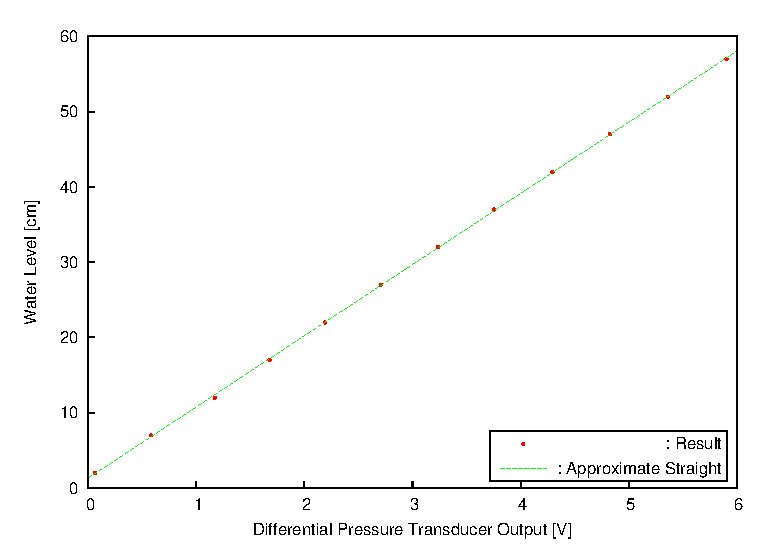
\includegraphics[width=0.9\hsize]{./fig/least_square.eps}
      \end{center}
      \caption{差圧変換器出力と水位の関係式}
      \label{fig:least_square}
    \end{figure}

  \subsection{流入量から差圧変換器出力への伝達関数}
    実験2の結果から,流入量を入力,差圧変換器出力を出力とした伝達関数$G_1(s)$を求める.
    図\ref{fig:data2dpt}が二次遅れ系の応答を示していることから,
    流入量から差圧変換器出力への伝達関数$G_1(s)$は式(2.2)から次のようにおける.
    \begin{equation}
      G_1(s) = \frac{V(S)}{U(S)} = \frac{K}{(1 + T_1 s)(1 + T_2 s)}
    \end{equation}
    ただし,流入量を$u(t)$,差圧変換器出力を$v(t)$とし,
    $U(s)$及び$V(s)$はそれぞれ$u(t)$,$v(t)$に対応するラプラス変換後の変数である.\\
    
    まず,この伝達関数$G_1(s)$について時定数$T_1$,$T_2$を求める.
    実験2の結果(表\ref{tab:data2}および図\ref{fig:data2dpt})について
    グラフの変曲点を求めるため,各データ値とその次のデータ値との差分を求めた.
    これをグラフに表したものを図\ref{fig:data2diff}に示す.
    図\ref{fig:data2diff}より最も差分の大きな点,
    つまり,図\ref{fig:data2dpt}の変曲点は明らかである.
    この点を変曲点$t_c = 170\,\mathrm{[sec]}$とした.
    なお,この時の差圧変換器出力は$2.488\,\mathrm{[V]}$である.\\

    \begin{figure}[b]
      \begin{center}
        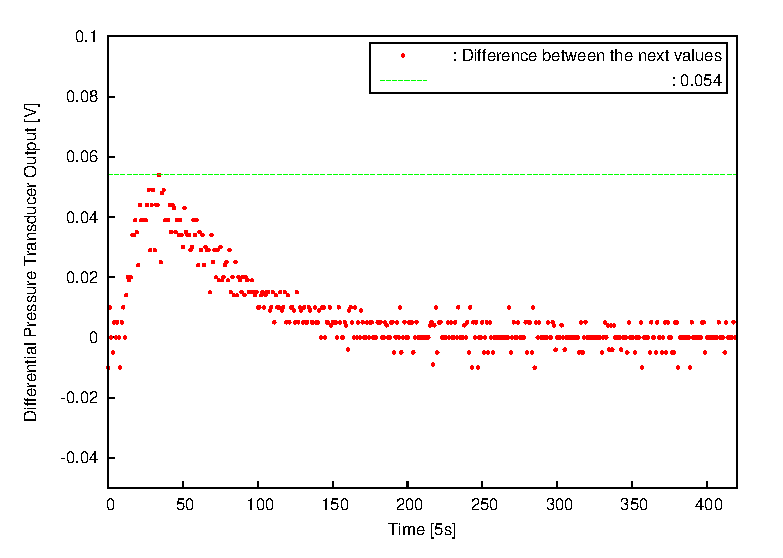
\includegraphics[width=0.9\hsize]{./fig/data2diff.eps}
      \end{center}
      \caption{差圧変換器出力各データ値の次の値との差分}
      \label{fig:data2diff}
    \end{figure}

    ここで,図\ref{fig:data2dpt}における
    変曲点$(170,2.488)$を通る傾き$a$の直線は$y = a x + 2.488 -34a$とおける.
    ここから最も点$(170,2.488)$の接線に相応しいと思われる傾きaを設定し,
    それと$y = 1.707$,$y = 5.043$との交点をそれぞれ$t_a$,$t_b$とする.
    傾き$a = 0.04$と設定することで$t_a = 14.475 \times 5 \approx 72$,
    $t_b = 97.875 \times 5 \approx 489$となり,
    これらから$T_A$,$T_C$は以下のように求まった.
    \begin{eqnarray}
      T_A &=& t_b - t_a = 489 - 72 = 417 \\
      T_C &=& t_b - t_c = 489 - 170 = 319
    \end{eqnarray}
    以上の接線について,図\ref{fig:data2lines}に示す.\\
    
    \begin{figure}[b]
      \begin{center}
        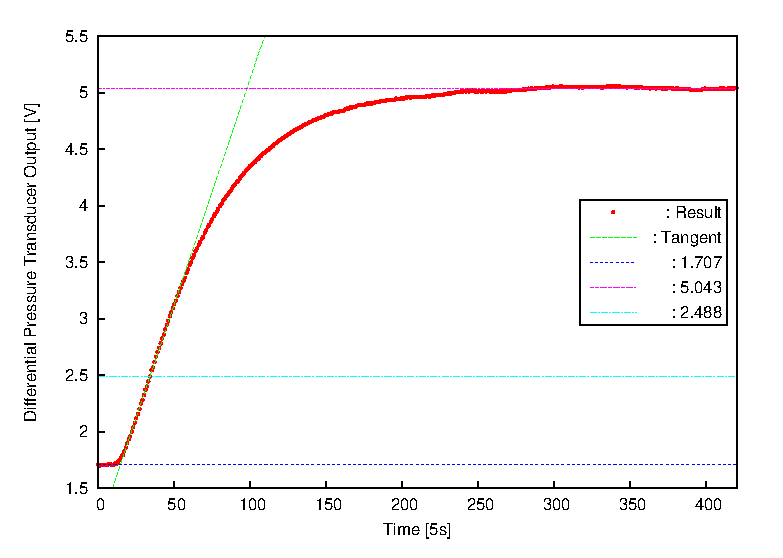
\includegraphics[width=0.9\hsize]{./fig/data2lines.eps}
      \end{center}
      \caption{変曲点および接線の推定}
      \label{fig:data2lines}
    \end{figure}
    
    さらに,式(2.16)のように定義すると$\alpha \approx 0.765$となる.
    式(2.18),(2.19)より,これらの交点座標$x_1$,$x_2$を用いることで
    $T_1$と$T_2$は次のように求まる.
    \begin{eqnarray}
      T_1 = T_A \times x_1 \\
      T_2 = T_A \times x_2 
    \end{eqnarray}
    ここで,式(2.19)は解析的に解を求めることが出来ないため,
    表\ref{tab:log}のデータをプロットし,
    $y = 0.765 - x$との交点座標$x_1$,$x_2$は
    以上の式を満たすよう目分量にて決定した.
    交点座標$x_1$,$x_2$の決定について,推定の補助として用いた直線と
    式(2.18),(2.19)をグラフに表したものを図\ref{fig:datalog}に示す.

    \begin{figure}[b]
      \begin{center}
        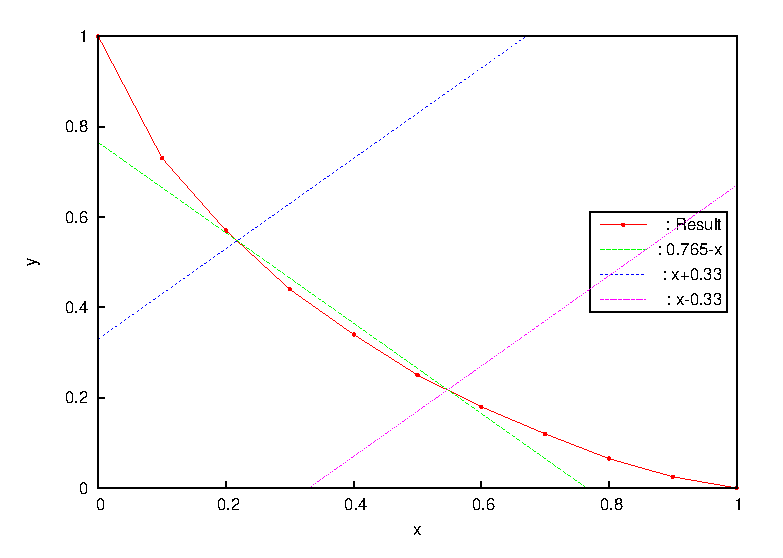
\includegraphics[width=0.9\hsize]{./fig/datalog.eps}
      \end{center}
      \caption{交点座標$x_1$,$x_2$の推定}
      \label{fig:datalog}
    \end{figure}

    図\ref{fig:datalog}中の直線より,
    交点座標は$x_1 = 0.2175$,$x_2 = 0.5475$と求まり,
    $T_1 = 90.6975 \approx 90.70$,$T_2 = 228.3075 \approx 228.3$である.\\

    次に,伝達関数$G_1(s)$のゲイン$K$を求める.
    大きさ$r$のステップ入力を加えた時の時間応答$h(t)$は式(2.3)より
    \begin{equation}
      h(t) = r K \biggl( 1 + \frac{T_1}{T_2 - T_1} e^{- \frac{t}{T_1}}
                           - \frac{T_2}{T_2 - T_1} e^{- \frac{t}{T_2}} \biggr)
    \end{equation}
    である.$t \rightarrow \infty$とすると,図\ref{fig:data2lines}より
    \begin{equation}
      h(\infty) = r K = 5.043
    \end{equation}
    となり,また$r = (23.5 -16.9) \div 60 = 0.11$であることから,ゲイン$K$は
    \begin{equation}
      K = 5.043 \div 0.11 \approx 45.85
    \end{equation}
    である.\\
    
    よって求める伝達関数$G_1(s)$は
    \begin{equation}
      G_1(s) = \frac{V(s)}{U(s)} = \frac{45.85}{(1 + 90.70 s)(1 + 228.3)}
    \end{equation}
    である.\\
    
  \subsection{流入量から水位への伝達関数}
    実験1および2の結果から,流入量を入力,
    タンク2の水位を出力とした伝達関数$G_2(s)$を求める.
    伝達関数は初期値を0と置くため,式(6.4)より
    \begin{equation}
      v(t) = 0.1058 h(t)
    \end{equation}
    とおける.この式をラプラス変換することで
    \begin{equation}
      V(s) = 0.1058 H(s)
    \end{equation}
    を得る.
    ただし,$H(s)$及び$V(s)$はそれぞれ$h(t)$,
    $v(t)$に対応するラプラス変換後の変数である.\\
    以上より,伝達関数$G_2(s)$は
    \begin{equation}
      G_2(s) = \frac{H(s)}{U(s)} = \frac{H(s)}{V(s)} G_1(s)
             \approx \frac{433.4}{(1 + 90.70 s)(1 + 228.3)}
    \end{equation}
    である.
    
  \subsection{同定した伝達関数の妥当性}
    以上で同定した伝達関数の妥当性について検討する.
    前項で求めた伝達関数$G_2(s)$に大きさ$r = 0.11$の
    ステップ入力を加えた時の時間応答は,
    \begin{equation}
      h(t) = 47.67 (1 + 0.6592 e^{- \frac{t}{90.7}} - 1.659 e^{- \frac{t}{228.3}})
    \end{equation}
    である.
    式(6.4)と実験2より得られたデータを用いて求めた時間-水位の
    実験結果と,式(6.17)の時間応答についてグラフに表したものを
    図\ref{fig:data4}に示す.
    また,100秒毎のそれぞれの値と相対誤差を表\ref{tab:data4}に示す.\\

    \begin{figure}[b]
      \begin{center}
        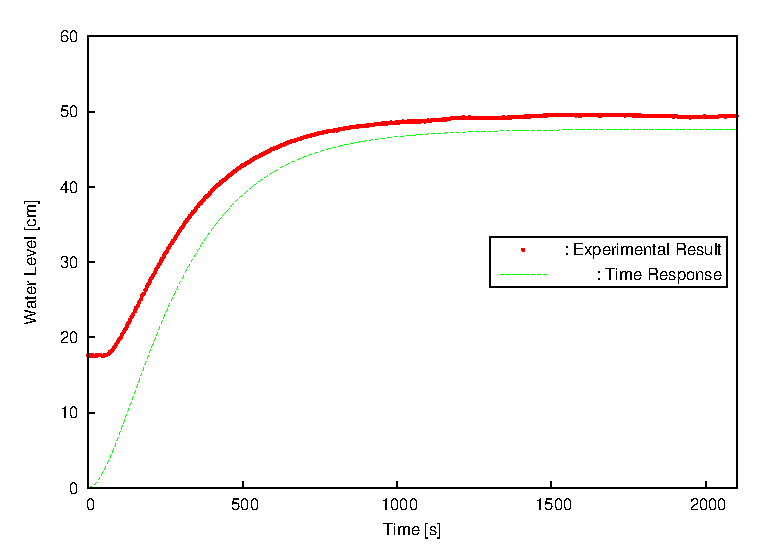
\includegraphics[width=0.9\hsize]{./fig/data4dpt.eps}
      \end{center}
      \caption{実験値と同定結果の比較}
      \label{fig:data4}
    \end{figure}

    \begin{table}[h]
  \begin{center}
    \caption{実験値と同定結果の相対誤差}
    \begin{tabular}{|c|c|c|c|} \hline
      時間$\mathrm{[sec]}$ & 水位$\mathrm{[cm]}$ & 同定結果$\mathrm{[cm]}$ & 相対誤差$\mathrm{[\%]}$ \\ \hline \hline
0    & 17.61 & 17.62 &  0.02 \\ \hline
100  & 19.76 & 22.79 & 15.34 \\ \hline
200  & 27.49 & 30.95 & 12.60 \\ \hline
300  & 34.48 & 37.82 &  9.67 \\ \hline
400  & 39.47 & 42.78 &  8.38 \\ \hline
500  & 42.87 & 46.16 &  7.67 \\ \hline
600  & 45.06 & 48.39 &  7.39 \\ \hline
700  & 46.60 & 49.86 &  7.00 \\ \hline
800  & 47.52 & 50.81 &  6.91 \\ \hline
900  & 48.14 & 51.43 &  6.84 \\ \hline
1000 & 48.55 & 51.82 &  6.73 \\ \hline
1100 & 48.83 & 52.08 &  6.66 \\ \hline
1200 & 49.16 & 52.25 &  6.29 \\ \hline
1300 & 49.16 & 52.35 &  6.50 \\ \hline
1400 & 49.35 & 52.42 &  6.24 \\ \hline
1500 & 49.54 & 52.47 &  5.92 \\ \hline
1600 & 49.54 & 52.50 &  5.98 \\ \hline
1700 & 49.58 & 52.52 &  5.93 \\ \hline
1800 & 49.44 & 52.53 &  6.24 \\ \hline
1900 & 49.39 & 52.54 &  6.36 \\ \hline
2000 & 49.35 & 52.54 &  6.47 \\ \hline
2100 & 49.44 & 52.54 &  6.27 \\ \hline
    \end{tabular}
    \label{tab:data4}
  \end{center}
\end{table}


    図と表から,過渡状態は相対誤差が非常に大きく,
    定常状態付近ではおよそ4\%以内に収まっていることが読み取れるが,
    どちらも妥当ということは出来ない.
    ゲインを50付近に設定することで定常状態での値はほぼ一致させることができるが,
    過渡状態の誤差は依然として大きいままである.
    このことから,同定した伝達関数は実際よりもゲインが小さく,
    即応性が低い,つまり時定数も実際より小さいことが分かる.\\

    ゲインに誤差が生じた原因については,
    実験1の測定結果自体が殆ど線形であることから,
    実験装置,つまり水位の測定に用いたメジャーの不備が挙げられる.
    実際,実験装置に備え付けられていたメジャーはタンク2に対し
    完全に垂直であるとは言い難く,
    ここで誤差が生じることは実験中の時点で危惧されていたことである.\\

    時定数に誤差が生じた原因については,
    図5.3に対し目測で接線を設定したこと,
    計算に用いた式(2.19)に解析解がないためデータ点を用いたこと,
    また,そのグラフと直線の交点を目測で求めたことなど,
    人為的誤差が積み重なった結果だと考えられる.\\

\section{結論}
  レベル系の流入量を入力,水位を出力とした二次遅れ系の同定実験を行うことで,
  プロセス系への理解が充分に深まった.

\end{document}
